\documentclass[a4paper,9pt]{extarticle}

%=========================================================
% PACKAGES
%=========================================================

\usepackage[
a4paper,
top=1.8cm,
bottom=1.5cm,
footskip=7mm,
left=1cm,
right=1cm,
headheight=14pt,
headsep=5mm
]{geometry}
\usepackage[T1]{fontenc}
\usepackage[utf8]{inputenc}
\usepackage[french]{babel}

\usepackage[sfdefault]{FiraSans}
\renewcommand{\familydefault}{\sfdefault}

\usepackage{multicol}
\setlength{\columnsep}{0.7cm}

\usepackage{amsmath,amssymb}

\usepackage{titlesec}
\usepackage{enumitem}

\usepackage{tcolorbox}
\tcbuselibrary{skins,breakable}

\usepackage{xcolor}

\usepackage{graphicx}
\usepackage{float}

\usepackage{tikz}

\usepackage{fancyhdr}
\usepackage[hidelinks]{hyperref}


%=========================================================
% PAGE SETTINGS
%=========================================================

\setlength{\parindent}{0pt}
\setlength{\parskip}{1.5pt}

\setlength{\abovedisplayskip}{4pt}
\setlength{\belowdisplayskip}{4pt}

\setlist[itemize]{
leftmargin=*,
itemsep=1pt,
topsep=1pt
}


%=========================================================
% COLORS
%=========================================================

\definecolor{Blue}{HTML}{E3F0FF}
\definecolor{Green}{HTML}{E3F7EA}
\definecolor{Pink}{HTML}{FFE5ED}
\definecolor{Orange}{HTML}{FFF0DC}
\definecolor{Purple}{HTML}{EEE7FF}
\definecolor{Yellow}{HTML}{FFFADB}


\definecolor{BlueTitle}{HTML}{285B8F}
\definecolor{GreenTitle}{HTML}{287052}
\definecolor{PinkTitle}{HTML}{A84063}
\definecolor{OrangeTitle}{HTML}{A96500}
\definecolor{PurpleTitle}{HTML}{6245A5}


%=========================================================
% HEADER
%=========================================================

\pagestyle{fancy}

\fancyhf{}

\fancyhead[L]{\small\textbf{Game Theory and Strategic Decisions}}
\fancyhead[C]{\small Introduction and Nash Equilibrium}
\fancyhead[R]{\small Week 01 --- 07-13/09/2026}

\fancyfoot[C]{\small\href{https://github.com/AlphaXT38G/notes_ba5}{github.com/AlphaXT38G/notes\_ba5}}
\fancyfoot[R]{\small \thepage}

\renewcommand{\headrulewidth}{0.4pt}



%=========================================================
% TITLES
%=========================================================

\titleformat{\section}
{\large\bfseries\color{BlueTitle}}
{}{0pt}{}

\titlespacing{\section}
{0pt}{6pt}{3pt}


% separator

\newcommand{\separator}{
\vspace{2pt}
\hrule
\vspace{3pt}
}


%=========================================================
% BOXES
%=========================================================

% Boxes are kept whole (unbreakable): inside multicols, a box split by tcolorbox
% leaves an empty column behind it.

% DEFINITION - blue
\newtcolorbox{definition}{
enhanced,
unbreakable,
colback=Blue,
colframe=BlueTitle,
boxrule=0.7pt,
arc=0mm,
title=\textbf{Definition},
fonttitle=\bfseries
}

% IMPORTANT - pink
\newtcolorbox{important}{
enhanced,
unbreakable,
colback=Pink,
colframe=PinkTitle,
boxrule=0.7pt,
arc=0mm,
title=\textbf{Key idea},
fonttitle=\bfseries
}

% FORMULAS - green
\newtcolorbox{formula}{
enhanced,
unbreakable,
colback=Green,
colframe=GreenTitle,
boxrule=0.7pt,
arc=0mm,
title=\textbf{Key formulas},
fonttitle=\bfseries
}

% WARNING - orange
\newtcolorbox{warning}{
enhanced,
unbreakable,
colback=Orange,
colframe=OrangeTitle,
boxrule=0.7pt,
arc=0mm,
title=\textbf{Warning},
fonttitle=\bfseries
}

% EXAMPLE - purple
\newtcolorbox{example}{
enhanced,
unbreakable,
colback=Purple,
colframe=PurpleTitle,
boxrule=0.7pt,
arc=0mm,
title=\textbf{Example},
fonttitle=\bfseries
}

% SUMMARY - orange
\newtcolorbox{summary}{
enhanced,
unbreakable,
colback=Yellow,
colframe=OrangeTitle,
boxrule=0.7pt,
arc=0mm,
title=\textbf{Summary},
fonttitle=\bfseries
}



%=========================================================
% FIGURE BOX
%=========================================================

\newtcolorbox{figurebox}{
enhanced,
colback=white,
colframe=gray,
boxrule=0.5pt,
arc=0mm,
center
}



%=========================================================
% DOCUMENT
%=========================================================

\begin{document}

%\footnotesize   --> To reduce the size of the text

\thispagestyle{fancy}



\begin{multicols}{2}



%=========================================================
\section{Course Essentials}


\begin{summary}

\begin{itemize}

\item 14 lectures, on Tuesday from 1\string:15pm to 3pm (one 15-minute break around 2pm).

\item Assistant: Luiz Bissoto (\href{mailto:luiz.bissoto@epfl.ch}{luiz.bissoto@epfl.ch}).

\item Grading based on \textbf{3 problem sets}, weights \textbf{40\%, 40\%, 20\%}.
Assignments can be done in groups of up to 3 people.

\end{itemize}

\end{summary}


\textbf{Three parts of the course}

\begin{itemize}

\item Basics of non-cooperative game theory (approximately 7 lectures)

\item Auction theory with applications to Ebay and Google advertising auctions (approx.\ 4 lectures)

\item Evolutionary game theory (approx.\ 2 lectures)

\end{itemize}



%=========================================================
\section{Cooperative vs Non-Cooperative Games}


\begin{definition}

\textbf{NON-COOPERATIVE GAME}

There is \textbf{no external authority enforcing rules of cooperative behavior}.

Each player tries to maximize her benefit at any time, even by damaging others. Even when a
contract between two players could be beneficial to both, they cannot stipulate it, because
no authority is able to enforce it.

\end{definition}


\begin{definition}

\textbf{COOPERATIVE GAME}

Involves negotiation, bargaining, contracts,\dots

\end{definition}


\begin{important}

Classical game theory focuses on \textbf{non-cooperative games}: this is what we study in
this course.

\end{important}



%=========================================================
\section{What is a Game?}


\begin{definition}

\textbf{GAME}

A mathematical model of strategic interaction, defined by:

\begin{itemize}

\item \textbf{Players} -- people, businesses, countries\dots

\item \textbf{Choices} -- players make one or multiple choices between different possible
actions. A player's \textbf{strategy} is her rule for choosing actions.

\item \textbf{Outcomes} -- when players have made their choices, an outcome is realized
and the game ends. An outcome is expressed in terms of a \textbf{payout} to the players
(e.g.\ Player 1 wins \$1, Player 2 loses \$2).

\end{itemize}

\end{definition}


\begin{important}

Common to all games: \textbf{ALL PLAYERS CARE ABOUT IS THEIR OWN PAYOUT!!}

\end{important}


\separator


\textbf{Elements distinguishing different types of game}

\begin{itemize}

\item \textbf{Timing} -- do players choose once (e.g.\ rock-paper-scissors) or repeatedly
over time (e.g.\ chess)? Does the game eventually end, or continue forever? Do they choose
\textbf{simultaneously} or in turn?

\item \textbf{Observation} -- can the players observe each other's choices?

\end{itemize}


\textbf{This week: the simplest type of games}

\begin{itemize}

\item 2 players;

\item each player makes one choice;

\item all choose simultaneously (so do not observe the other's action).

\end{itemize}



%=========================================================
\section{Normal Form Representation}


\begin{definition}

\textbf{NORMAL FORM}

A table with one row per action of Player 1, one column per action of Player 2, and in each
cell the payouts \textbf{(Player 1, Player 2)}.

\end{definition}


\begin{example}

\textbf{Rock-Paper-Scissors}

\begin{center}
\begin{tabular}{c|ccc}
$1 \backslash 2$ & R & P & S \\
\hline
R & (0,0) & (-1,1) & (1,-1) \\
P & (1,-1) & (0,0) & (-1,1) \\
S & (-1,1) & (1,-1) & (0,0) \\
\end{tabular}
\end{center}

\begin{itemize}

\item Players: 1, 2

\item Possible actions for Player 1 (and for Player 2): R(ock), P(aper), S(cissors).

\end{itemize}

\end{example}


\begin{formula}

Payout notation:

\[
\mathcal{P}^{(1)}(R,P) = -1
\]

Payout for Player 1 if 1 chooses R and 2 chooses P.

\[
\mathcal{P}^{(2)}(S,R) = 1
\]

Payout for Player 2 if 1 chooses S and 2 chooses R.

\end{formula}



%=========================================================
\section{Pure vs Mixed Strategies}


Player $i$ can choose between $M$ \textbf{actions} $(a_1^{(i)}, a_2^{(i)}, \dots, a_M^{(i)})$.


\begin{definition}

\textbf{MIXED STRATEGY}

An $M$-component vector

\[
s^{(i)} = (p_1^{(i)}, p_2^{(i)}, \dots, p_M^{(i)})
\]

with $0 \le p_j^{(i)} \le 1$ for $j = 1, \dots, M$ and $\sum_{j=1}^{M} p_j^{(i)} = 1$.

Each component $j$ is the probability of choosing action $a_j^{(i)}$.

\textbf{Different players choose their actions independently.}

\end{definition}


\begin{definition}

\textbf{PURE STRATEGY}

A vector with one component equal to one, and the others equal to zero.

\end{definition}



%=========================================================
\section{Actions vs Strategies}


\begin{warning}

\begin{itemize}

\item \textbf{Action} (letter $a$): what a player ends up playing.

\item \textbf{Strategy} (letter $s$): the $M$-component vector containing the
\emph{ex-ante} probability of playing each of the different actions.

\end{itemize}

\end{warning}


\begin{important}

When players use mixed strategies, their objective is to maximize their \textbf{expected
payout}.

Expected value of a random variable: weighted average over possible outcomes, weighed with
their respective probabilities.

\end{important}


\begin{formula}

2 players, each choosing between actions $A$ and $B$:
$s^{(1)} = (p_A^{(1)}, p_B^{(1)})$, $s^{(2)} = (p_A^{(2)}, p_B^{(2)})$.

\begin{align*}
E[\mathcal{P}^{(1)}(s^{(1)}, s^{(2)})] ={}& Prob(A,A)\,\mathcal{P}^{(1)}(A,A) \\
&+ Prob(A,B)\,\mathcal{P}^{(1)}(A,B) \\
&+ Prob(B,A)\,\mathcal{P}^{(1)}(B,A) \\
&+ Prob(B,B)\,\mathcal{P}^{(1)}(B,B)
\end{align*}

The choices are independent: $Prob(A,A) = p_A^{(1)} p_A^{(2)}$,
$Prob(A,B) = p_A^{(1)} p_B^{(2)}$, etc. Hence

\begin{align*}
E[\mathcal{P}^{(1)}(s^{(1)}, s^{(2)})] ={}& p_A^{(1)} p_A^{(2)} \mathcal{P}^{(1)}(A,A) \\
&+ p_A^{(1)} p_B^{(2)} \mathcal{P}^{(1)}(A,B) \\
&+ p_B^{(1)} p_A^{(2)} \mathcal{P}^{(1)}(B,A) \\
&+ p_B^{(1)} p_B^{(2)} \mathcal{P}^{(1)}(B,B)
\end{align*}

\end{formula}


\begin{important}

In the simultaneous-move games of this week, each player \textbf{knows the other players'
strategy, but not their actions}.

\end{important}


\begin{example}

In Rock-Paper-Scissors, I may know that my opponent plays the three actions with probability
$(0.3, 0.3, 0.4)$ -- e.g.\ because we already played together many times -- but I don't know
what she will play this time.

\end{example}



%=========================================================
\section{Nash Equilibrium}


\begin{definition}

\textbf{NASH EQUILIBRIUM (NE)}

The most widely used \textbf{solution concept}.

Given a game with $N$ players, a \textbf{strategy profile} (the set of the strategies taken
by each of the players) $(s^{(1)}, s^{(2)}, \dots, s^{(N)})$ is a Nash equilibrium iff the
payout of each player $i$ is such that

\[
\mathcal{P}^{(i)}(s^{(i)}, s^{(-i)}) \ge \mathcal{P}^{(i)}(\tilde{s}^{(i)}, s^{(-i)})
\quad \text{for every possible } \tilde{s}^{(i)}
\]

where $s^{(-i)}$ denotes the strategies of all players \emph{other than} $i$.

\end{definition}


\begin{important}

A NE is the best that one player can do \emph{given the strategies of all the other
players}.

\end{important}


\separator


\textbf{Pure-strategy Nash equilibrium}

NE obtained when we restrict ourselves to the case in which all players adopt pure strategies
(i.e.\ always play the same action): a profile in which the action of each player is the
\textbf{best response} to the action of the other players.


\begin{example}

\begin{center}
\begin{tabular}{c|cc}
$1 \backslash 2$ & L & R \\
\hline
U & (8,7) & (4,6) \\
D & (6,5) & (7,8) \\
\end{tabular}
\end{center}

\begin{itemize}

\item \textbf{Player 1}: if 2 moves Left, 1 should move Up; if 2 moves Right, 1 should
move Down.

\item \textbf{Player 2}: if 1 moves Up, 2 should move Left; if 1 moves Down, 2 should
move Right.

\end{itemize}

Circling each best response, the cells where both payouts are circled are the NE:

\begin{center}

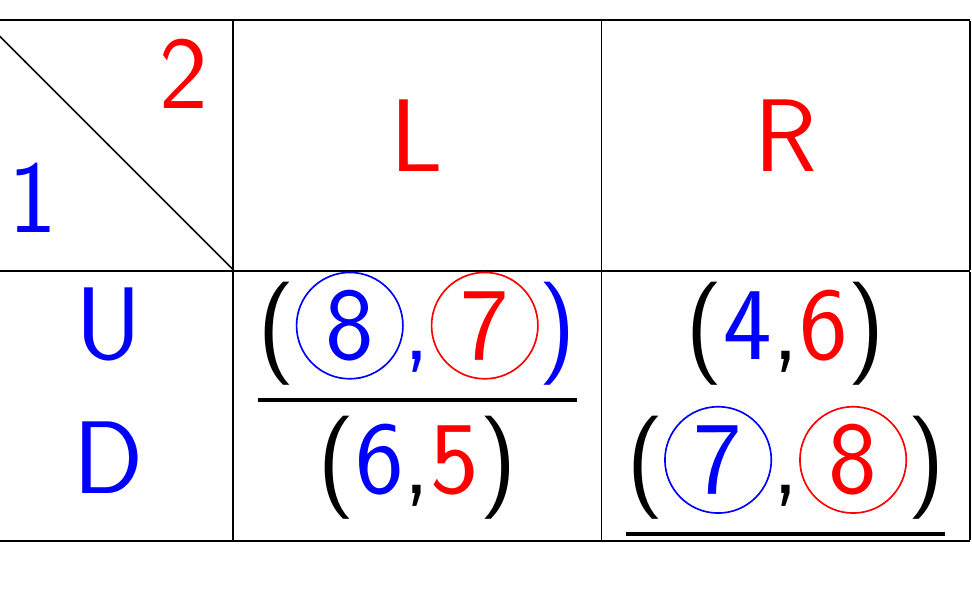
\includegraphics[
width=0.6\linewidth
]{../images/week01_01.png}

\end{center}

\textbf{2 NE}: $(U,L)$ and $(D,R)$.

\end{example}


\begin{warning}

Game with two equilibria: the theory cannot tell which one will be chosen.

\end{warning}



\end{multicols}


\end{document}
